\section{Materiais e Métodos}
\label{sec:metodologia}

O trabalho é computacional. Ele usa dados secundários e públicos, implementa modelos de equações
diferenciais em R e compara as simulações com a série de notificações e com o inquérito sorológico do
Recife. Todo o código fica num repositório aberto e um script regenera as figuras e tabelas conferindo os
resultados contra as expressões analíticas, o que torna cada número deste documento reproduzível.

\subsection{Arcabouço Teórico/Tecnológico}

\paragraph{O modelo SEIR-SEI.} A população humana, de tamanho $N_h$ fechado, passa por suscetíveis $S_h$,
expostos $E_h$, que estão infectados mas ainda não transmitem, infectados $I_h$ e recuperados $R_h$. Os
mosquitos, em número $N_v = m N_h$, passam por suscetíveis $S_v$, expostos $E_v$, durante a incubação do
vírus, e infectantes $I_v$, que transmitem até morrer. Os mosquitos nascem e morrem na taxa $\mu_v$. Na
notação de Ross e Macdonald \cite{smith2012}, $a$ é o número de picadas por mosquito por dia, $b$ a
probabilidade de a picada de um mosquito infectante infectar o humano e $c$ a probabilidade de um humano
infectado infectar o mosquito que o pica. A Figura \ref{fig:diagrama} mostra a estrutura.

\begin{align}
\frac{dS_h}{dt} &= -a b \frac{I_v}{N_h} S_h, &
\frac{dE_h}{dt} &= a b \frac{I_v}{N_h} S_h - \sigma_h E_h, \nonumber\\
\frac{dI_h}{dt} &= \sigma_h E_h - \gamma I_h, &
\frac{dR_h}{dt} &= \gamma I_h, \nonumber\\
\frac{dS_v}{dt} &= \mu_v N_v - a c \frac{I_h}{N_h} S_v - \mu_v S_v, &
\frac{dE_v}{dt} &= a c \frac{I_h}{N_h} S_v - (\sigma_v + \mu_v) E_v, \nonumber\\
\frac{dI_v}{dt} &= \sigma_v E_v - \mu_v I_v. & &
\label{eq:seirsei}
\end{align}

\begin{figure}[htbp]
\centering
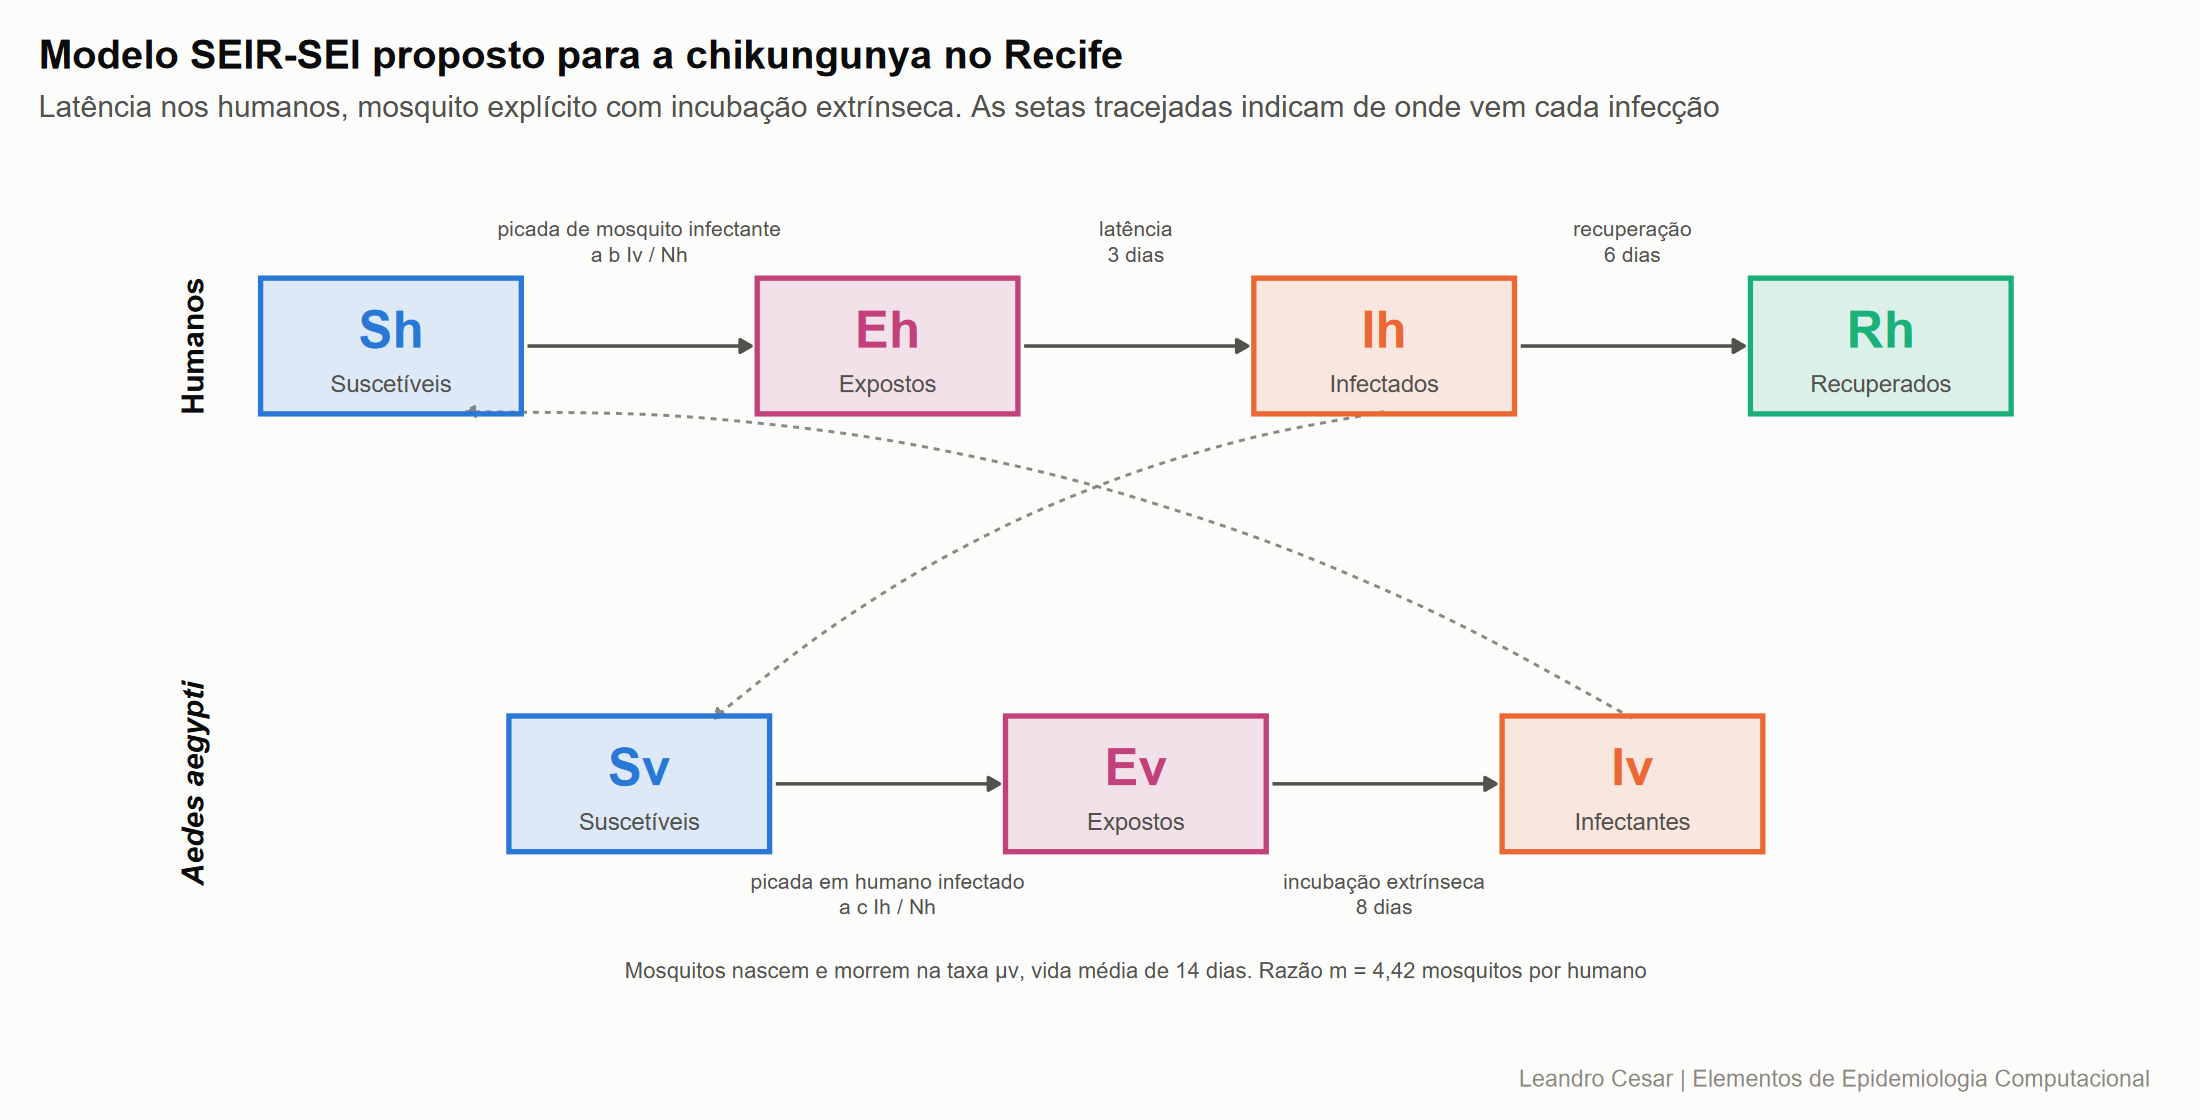
\includegraphics[width=\textwidth]{fig15_diagrama_seir_sei.png}
\caption{Estrutura do modelo SEIR-SEI com os parâmetros da Tabela \ref{tab:parametros}.}
\label{fig:diagrama}
\end{figure}

\paragraph{Parâmetros.} A Tabela \ref{tab:parametros} reúne os valores de partida. Eles vêm da compilação
de \citeonline{manore2014} para o \textit{Aedes aegypti}, com duas fontes adicionais: a latência humana
coincide com a mediana de \citeonline{rudolph2014}, e a incubação no mosquito é a média estimada por
\citeonline{christofferson2014} para a linhagem ECSA.

\begin{table}[htbp]
\centering
\caption{Parâmetros de partida do modelo SEIR-SEI.}
\label{tab:parametros}
\footnotesize
\begin{tabular}{p{5.4cm}llp{4.4cm}}
\toprule
\textbf{Parâmetro} & \textbf{Valor} & \textbf{Faixa} & \textbf{Fonte} \\
\midrule
$a$, picadas por mosquito por dia & 0,5 & 0,33 a 1 & \citeonline{manore2014} \\
$b$, infecção do mosquito para o humano & 0,24 & 0,001 a 0,35 & \citeonline{manore2014} \\
$c$, infecção do humano para o mosquito & 0,24 & 0,005 a 0,35 & \citeonline{manore2014} \\
$1/\sigma_h$, latência humana & 3 dias & 2 a 4 & \citeonline{manore2014, rudolph2014} \\
$1/\gamma$, período infeccioso humano & 6 dias & 3 a 7 & \citeonline{manore2014} \\
$1/\sigma_v$, incubação no mosquito & 8 dias & 3,8 a 14,5 & \citeonline{christofferson2014} \\
$1/\mu_v$, vida média do mosquito & 14 dias & 8 a 42 & \citeonline{manore2014} \\
$m$, mosquitos por humano & 4,42 & & escolhido para $R_{hh} = 3{,}4$ \\
\bottomrule
\end{tabular}
\end{table}

\paragraph{Números de reprodução.} Uma volta completa da transmissão tem duas metades. Um humano infectado
infecta, em média, $R_{vh} = a c m / \gamma$ mosquitos. Um mosquito recém infectado sobrevive à incubação com
probabilidade $\sigma_v/(\sigma_v + \mu_v)$ e depois pica durante $1/\mu_v$ dias, infectando
$R_{hv} = a b \sigma_v / ((\sigma_v + \mu_v)\mu_v)$ humanos. O produto $R_{hh} = R_{hv} R_{vh}$ é o número de
humanos infectados por um humano, depois de uma volta pelo mosquito. Ele corresponde ao $R_0$ de um modelo
SIR e determina o tamanho final do surto. O $R_0$ da matriz de próxima geração é $\sqrt{R_{hh}}$
\cite{manore2014}. Como a densidade de mosquitos por pessoa não é medida, $m$ foi escolhido para que
$R_{hh}$ seja 3,4, a média de \citeonline{haider2020}. Com os valores da Tabela \ref{tab:parametros},
$R_{vh} = 3{,}18$, $R_{hv} = 1{,}07$ e o $R_0$ de próxima geração é 1,84.

\paragraph{Tecnologia.} Os modelos são integrados em R 4.5.1 \cite{rcore2025} com o pacote
\texttt{deSolve} \cite{soetaert2010}. O código segue a estrutura dos cadernos do curso da disciplina e
separa modelo, integração, métricas, cenários, dados e figuras em arquivos próprios.

\subsection{Dados}

\paragraph{Notificações.} O portal de dados abertos da Prefeitura do Recife publica um arquivo por ano com
as notificações de chikungunya de 2015 a 2025 \cite{recife2026}. Apesar do nome ``casos confirmados'',
cada arquivo traz todas as notificações, com a classificação final. A série usada é a de \textbf{casos
prováveis}, a definição do Ministério da Saúde: todas as notificações de residentes no Recife, exceto as
descartadas, agregadas pela semana de início dos sintomas. Os arquivos de 2015 e 2016 trazem os códigos 1 e
2 na classificação final, que não constam no dicionário do portal. Eles foram mantidos como prováveis, e o
significado deles será confirmado com a vigilância municipal no OE2.

\paragraph{População.} Censo Demográfico 2022 do IBGE: 1.488.920 habitantes \cite{ibge2022}. As populações
por bairro e por distrito sanitário, necessárias ao OE4, também virão do Censo.

\paragraph{Sorologia.} O inquérito domiciliar de \citeonline{braga2023}, com 2.070 moradores de 5 a 65 anos
examinados entre agosto de 2018 e fevereiro de 2019, mediu IgG contra o vírus em 35,7\% (intervalo de
confiança de 95\% de 32,6\% a 38,9\%), com 22,3\%, 39,8\% e 38,6\% nos estratos alto, intermediário e baixo.

\subsection{Procedimentos por Objetivo}

\paragraph{OE1. Formular o modelo.} O sistema da Equação \ref{eq:seirsei} já está implementado. A taxa de
crescimento inicial é o maior autovalor do sistema linearizado dos compartimentos infectados no
equilíbrio sem doença, e a eficácia crítica do controle de criadouros é $1 - 1/R_{hh}$, porque $R_{hh}$ é
proporcional a $m$. O código confere a conservação das populações, a taxa de crescimento simulada contra o
autovalor e a ausência de surto com $R_{hh} < 1$.

\paragraph{OE2. Organizar os dados.} O script de download resolve os arquivos pela interface do portal,
guarda os dados brutos fora do repositório e produz a série semanal de casos prováveis para a cidade e
para cada distrito sanitário. Serão confirmados com a vigilância o significado dos códigos antigos e a
correspondência dos códigos de distrito.

\paragraph{OE3. Calibrar a primeira onda.} Os casos prováveis da semana $t$, $C_t$, serão modelados como
uma variável binomial negativa com média $\rho\, \Delta_t$, em que $\Delta_t$ é o número de humanos que
passam a infectados na semana e $\rho$ é a fração de notificação. A densidade de mosquitos vai variar ao
longo do ano, $m(t) = \bar{m}\,[1 + \delta \cos(2\pi(t - \phi)/365)]$, para representar a estação. Serão
estimados $\bar{m}$ (e portanto $R_{hh}$), $\rho$, $\delta$, $\phi$, a dispersão e a data de introdução,
por máxima verossimilhança. O inquérito entra como um segundo termo da verossimilhança: o modelo precisa
prever, para o período da coleta, a fração com anticorpos observada nos 2.070 examinados. Os intervalos
de confiança virão da verossimilhança perfilada. Séries de temperatura e chuva do INMET serão testadas
como alternativa à função cosseno.

\paragraph{OE4. Representar a heterogeneidade.} A população será dividida em grupos, por distrito sanitário
ou pelos três estratos do inquérito, cada um com sua densidade de mosquitos. A mistura entre grupos será
descrita por uma matriz com um parâmetro de acoplamento $\varepsilon$, de $\varepsilon = 0$, grupos
isolados, a $\varepsilon = 1$, mistura homogênea. O teste é se o modelo por grupos consegue reproduzir ao
mesmo tempo a série de 2015 e 2016, os 36\% do inquérito com a diferença entre estratos, e uma segunda onda
em 2021 sem supor perda de imunidade.

\paragraph{OE5. Avaliar o controle.} Com o modelo calibrado, serão simulados cenários de redução de
criadouros, que diminui o nascimento de mosquitos, e de aumento da mortalidade dos adultos, com eficácias
e datas de início diferentes, inclusive em relação à estação. O resultado de cada cenário é a taxa de
ataque, o pico e o número de casos evitados.

\paragraph{OE6. Divulgar.} O repositório reúne código, dados agregados, notebooks e o script de
conferência. Um painel vai mostrar a série observada, o ajuste do modelo e os cenários, com atualização a
cada novo arquivo anual do portal.

\subsection{Resultados Preliminares}
\label{sec:preliminares}

\subsubsection{O modelo SIR revisado}

O SIR da etapa anterior foi revisado depois da avaliação da professora (Anexo \ref{sec:anotacoes}). Com
$N = 1.488.920$, um caso inicial, período infeccioso de 6 dias \cite{manore2014} e $R_0 = 3{,}4$
\cite{haider2020}, a taxa de contágio é $\beta = R_0 \gamma = 0{,}567$ por dia. O pico acontece no dia 38,
com 438.146 suscetíveis, 515.090 infectados e 535.684 recuperados. A Tabela \ref{tab:validacao} confere a
simulação contra as três expressões analíticas do SIR. A taxa de ataque final não tem fórmula fechada e é
a raiz de $1 - a = e^{-R_0 a}$, encontrada numericamente. Simulação e raiz coincidem até a sexta casa
decimal.

\begin{table}[htbp]
\centering
\caption{Conferência do SIR contra a teoria.}
\label{tab:validacao}
\small
\begin{tabular}{lllll}
\toprule
\textbf{Grandeza} & \textbf{Expressão} & \textbf{Simulado} & \textbf{Analítico} & \textbf{Erro} \\
\midrule
Infectados no pico & $N\,(1 - (1 + \ln R_0)/R_0)$ & 515.089,7 & 515.089,5 & $4{,}5 \times 10^{-7}$ \\
Suscetíveis no pico & $N / R_0$ & 438.146,9 & 437.917,6 & $5{,}2 \times 10^{-4}$ \\
Taxa de ataque final & raiz de $1 - a = e^{-R_0 a}$ & 0,9620277 & 0,9620275 & $1{,}4 \times 10^{-7}$ \\
\bottomrule
\end{tabular}
\end{table}

Os dez cenários da Tabela \ref{tab:cenarios} cruzam as variações pedidas na atividade, taxas iguais e uma
taxa fixa com a outra variando, com os três regimes possíveis: $\beta > \gamma$, $\beta = \gamma$ e
$\gamma > \beta$.

\begin{table}[htbp]
\centering
\caption{Os dez cenários do SIR. Nos cenários sem surto, o desfecho é o total de pessoas infectadas até a
extinção.}
\label{tab:cenarios}
\footnotesize
\setlength{\tabcolsep}{4pt}
\resizebox{\textwidth}{!}{%
\begin{tabular}{clcrrrrrr}
\toprule
\textbf{N} & \textbf{Cenário} & \textbf{Regime} & $\beta$ & $\gamma$ & $R_0$ & \textbf{Pico} & \textbf{Infectados no pico} & \textbf{Desfecho} \\
\midrule
1 & Linha de base & $\beta > \gamma$ & 0,567 & 0,167 & 3,40 & dia 38 & 515.090 & 96,2\% \\
2 & Contágio 50\% maior & $\beta > \gamma$ & 0,850 & 0,167 & 5,10 & dia 23 & 720.957 & 99,4\% \\
3 & Contágio pela metade & $\beta > \gamma$ & 0,283 & 0,167 & 1,70 & dia 116 & 148.328 & 69,1\% \\
4 & Contágio igual à recuperação & $\beta = \gamma$ & 0,167 & 0,167 & 1,00 & sem surto & & 62 pessoas em 1 ano \\
5 & Contágio na metade da recuperação & $\gamma > \beta$ & 0,083 & 0,167 & 0,50 & sem surto & & 2 pessoas \\
6 & Período infeccioso dobrado & $\beta > \gamma$ & 0,567 & 0,083 & 6,80 & dia 33 & 847.936 & 99,9\% \\
7 & Recuperação igual ao contágio & $\beta = \gamma$ & 0,567 & 0,567 & 1,00 & sem surto & & 207 pessoas em 1 ano \\
8 & Recuperação acima do contágio & $\gamma > \beta$ & 0,567 & 0,708 & 0,80 & sem surto & & 5 pessoas \\
9 & Recuperação no dobro do contágio & $\gamma > \beta$ & 0,567 & 1,133 & 0,50 & sem surto & & 2 pessoas \\
10 & Mesmo $R_0$, ritmo pela metade & $\beta > \gamma$ & 0,283 & 0,083 & 3,40 & dia 76 & 515.090 & 96,2\% \\
\bottomrule
\end{tabular}}
\end{table}

Com $\gamma > \beta$, a pessoa se recupera, em média, antes de passar o vírus adiante. Enquanto quase todos
são suscetíveis, $I(t) = I_0 e^{(\beta - \gamma) t}$, que decai e vira uma reta numa escala logarítmica
(Figura \ref{fig:subcritico}). O total de infectados até a cadeia acabar é a soma $I_0(1 + R_0 + R_0^2 +
\dots) = I_0/(1 - R_0)$: 2 pessoas com $R_0 = 0{,}5$ e 5 com $R_0 = 0{,}8$, valores que a simulação reproduz.
Com $\beta = \gamma$ a prevalência fica parada e o total cresce em linha reta. Os cenários 5 e 9 têm o mesmo
$R_0$ e o mesmo total, mas o 9 se extingue mais rápido, assim como os cenários 1 e 10 têm o mesmo tamanho e
o 10 leva o dobro do tempo: a razão entre as taxas define o tamanho do surto, e a escala define a
velocidade. A Figura \ref{fig:fases} mostra a taxa de ataque para todas as combinações de $\beta$ e
$\gamma$.

\begin{figure}[htbp]
\centering
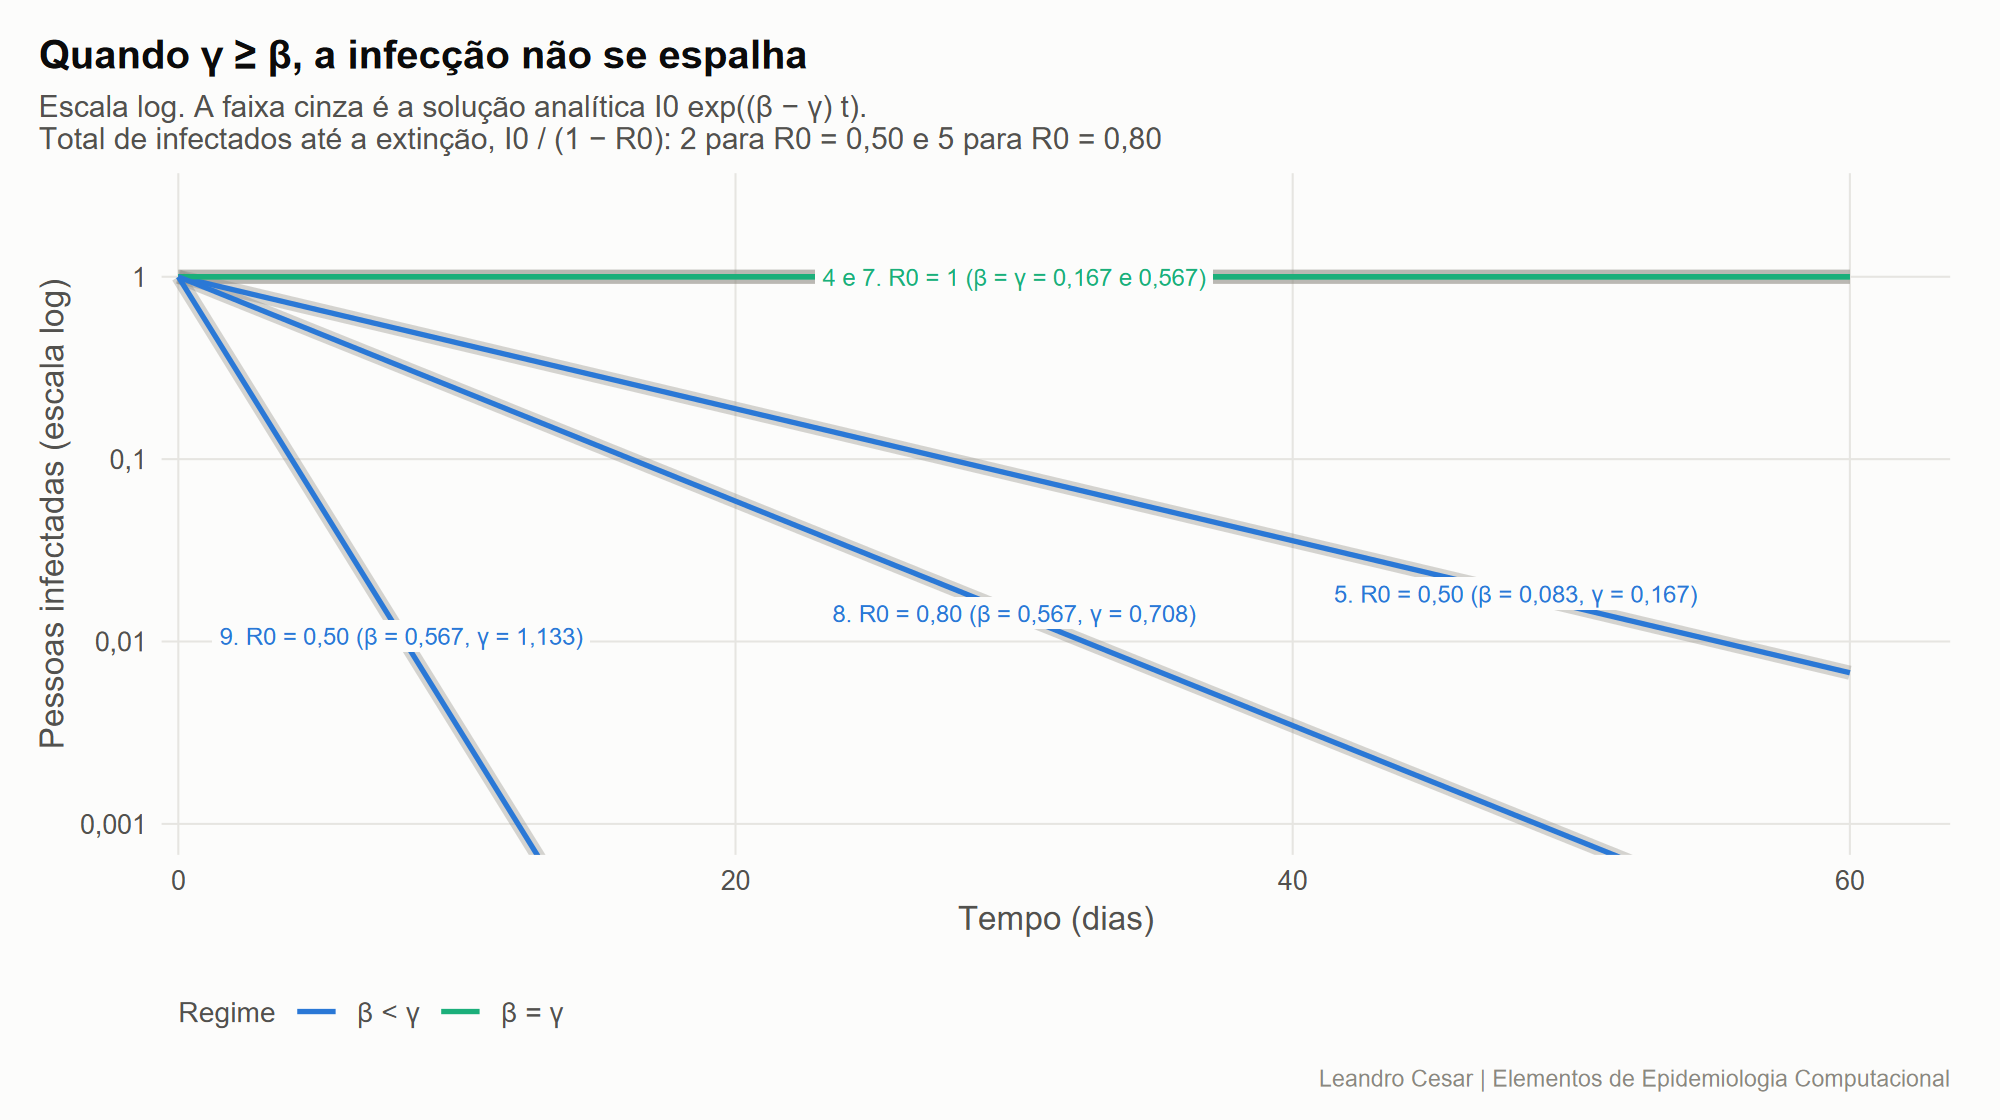
\includegraphics[width=0.92\textwidth]{fig06_regime_subcritico.png}
\caption{Cenários com $\gamma \geq \beta$ em escala logarítmica. A faixa cinza é a solução analítica.}
\label{fig:subcritico}
\end{figure}

\begin{figure}[htbp]
\centering
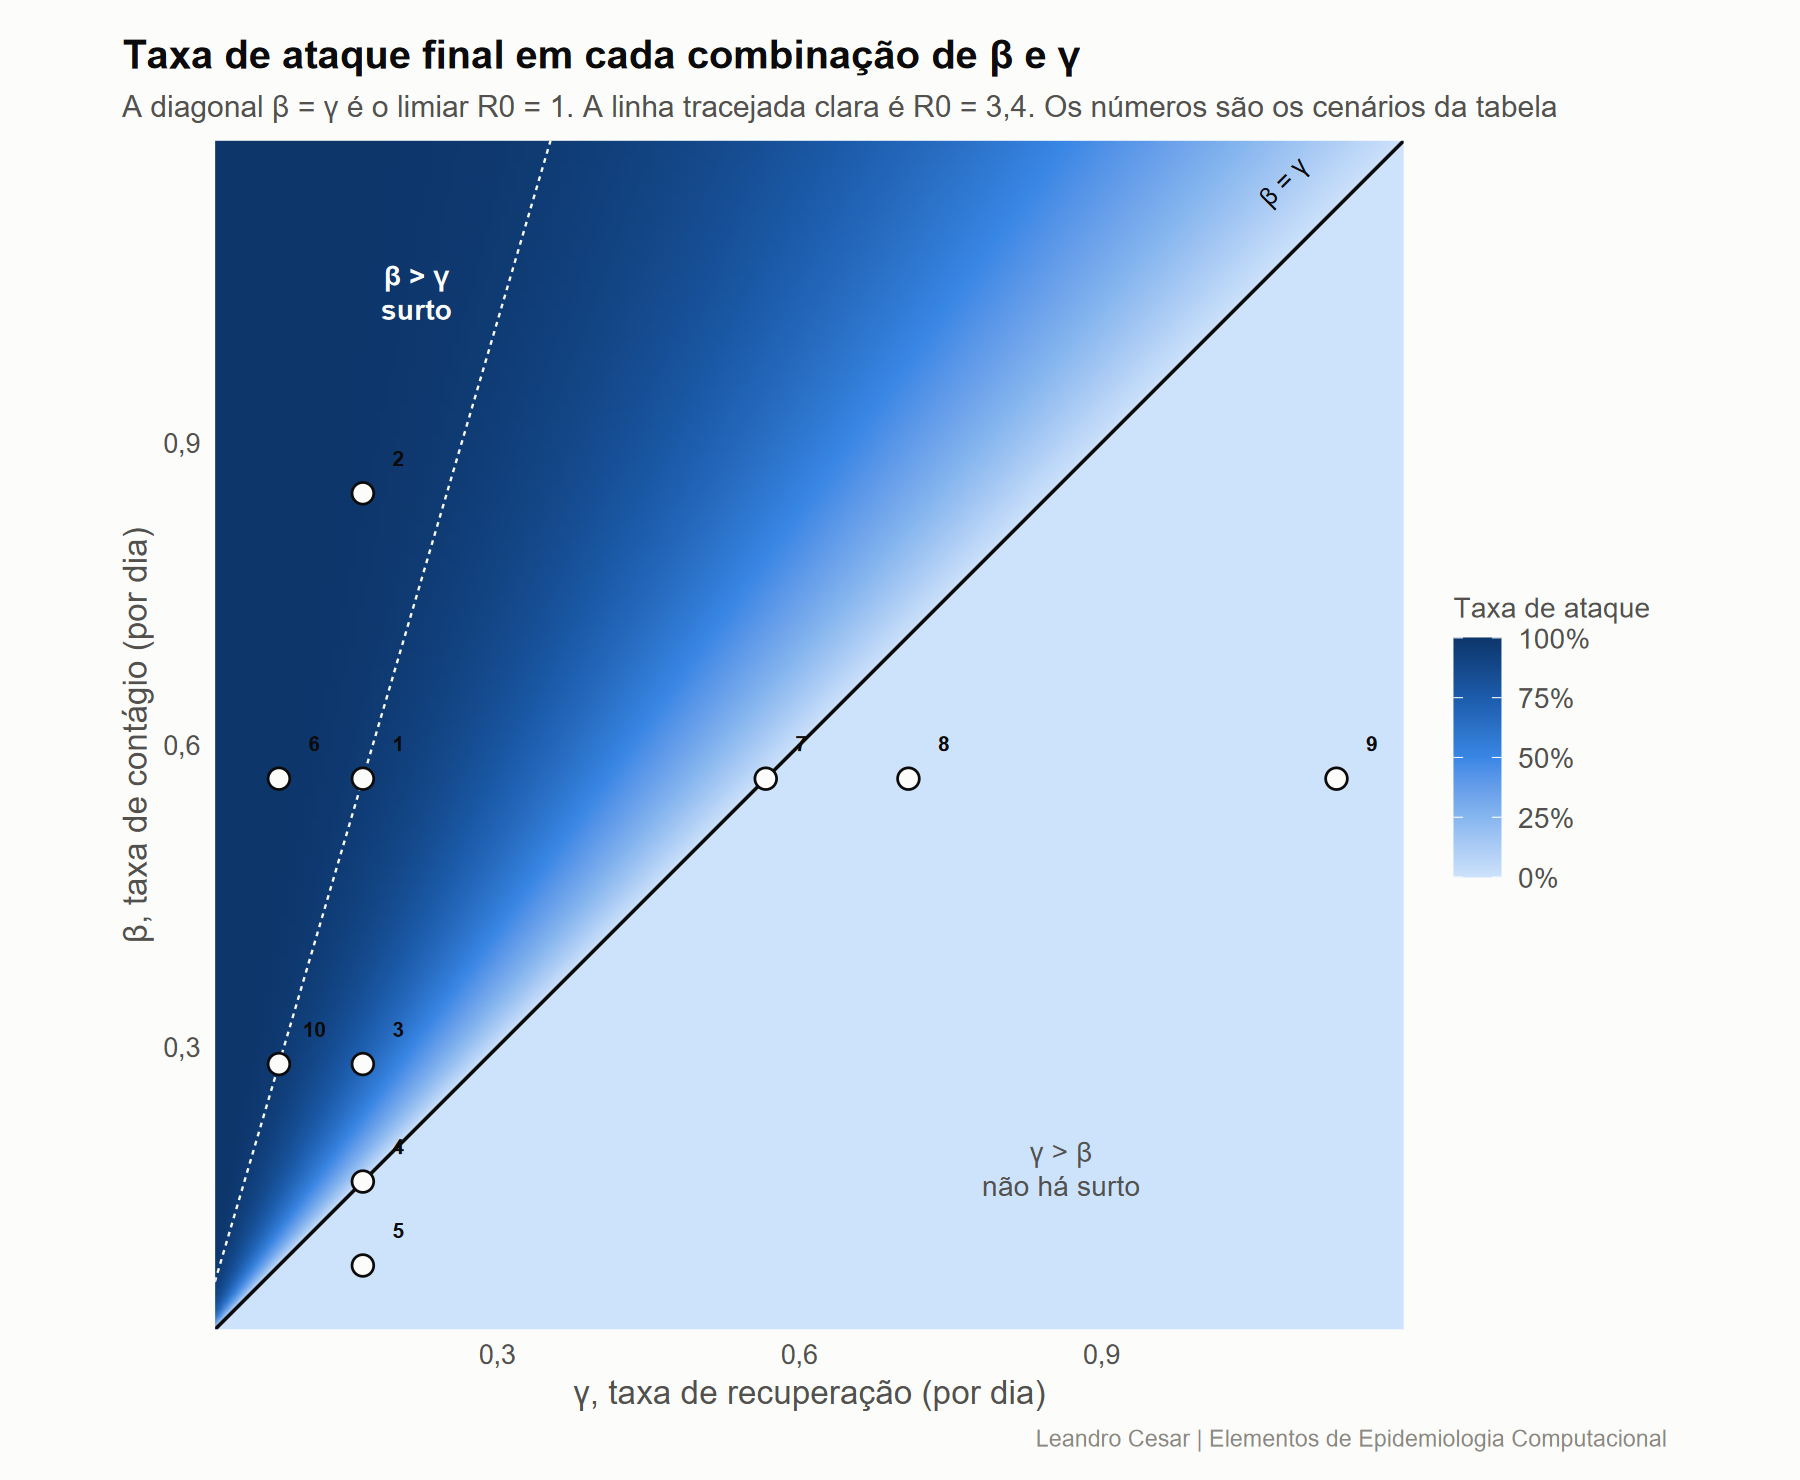
\includegraphics[width=0.8\textwidth]{fig07_mapa_fases.png}
\caption{Taxa de ataque final no plano $(\gamma, \beta)$. Abaixo da diagonal não há surto.}
\label{fig:fases}
\end{figure}

\paragraph{Controle vetorial no SIR.} Sem mosquito no modelo, o controle só pode ser uma redução de $\beta$,
o que se justifica porque a transmissão é proporcional à densidade de mosquitos \cite{smith2012}. Como não
há uma eficácia bem estabelecida para campanhas reais \cite{bowman2016}, a eficácia foi variada. Começando
no primeiro caso, o surto é evitado com redução de pelo menos $1 - 1/R_0 = 70{,}6\%$, entre 58,3\% e 76,2\%
na faixa de $R_0$ de 2,4 a 4,2. A Figura \ref{fig:inicio} varia também o dia de início. Uma redução de 80\%
evita o surto se começar no dia 0, deixa 24\% de infectados se começar no dia 30 e 84\% se começar no dia
40, logo depois do pico.

\begin{figure}[htbp]
\centering
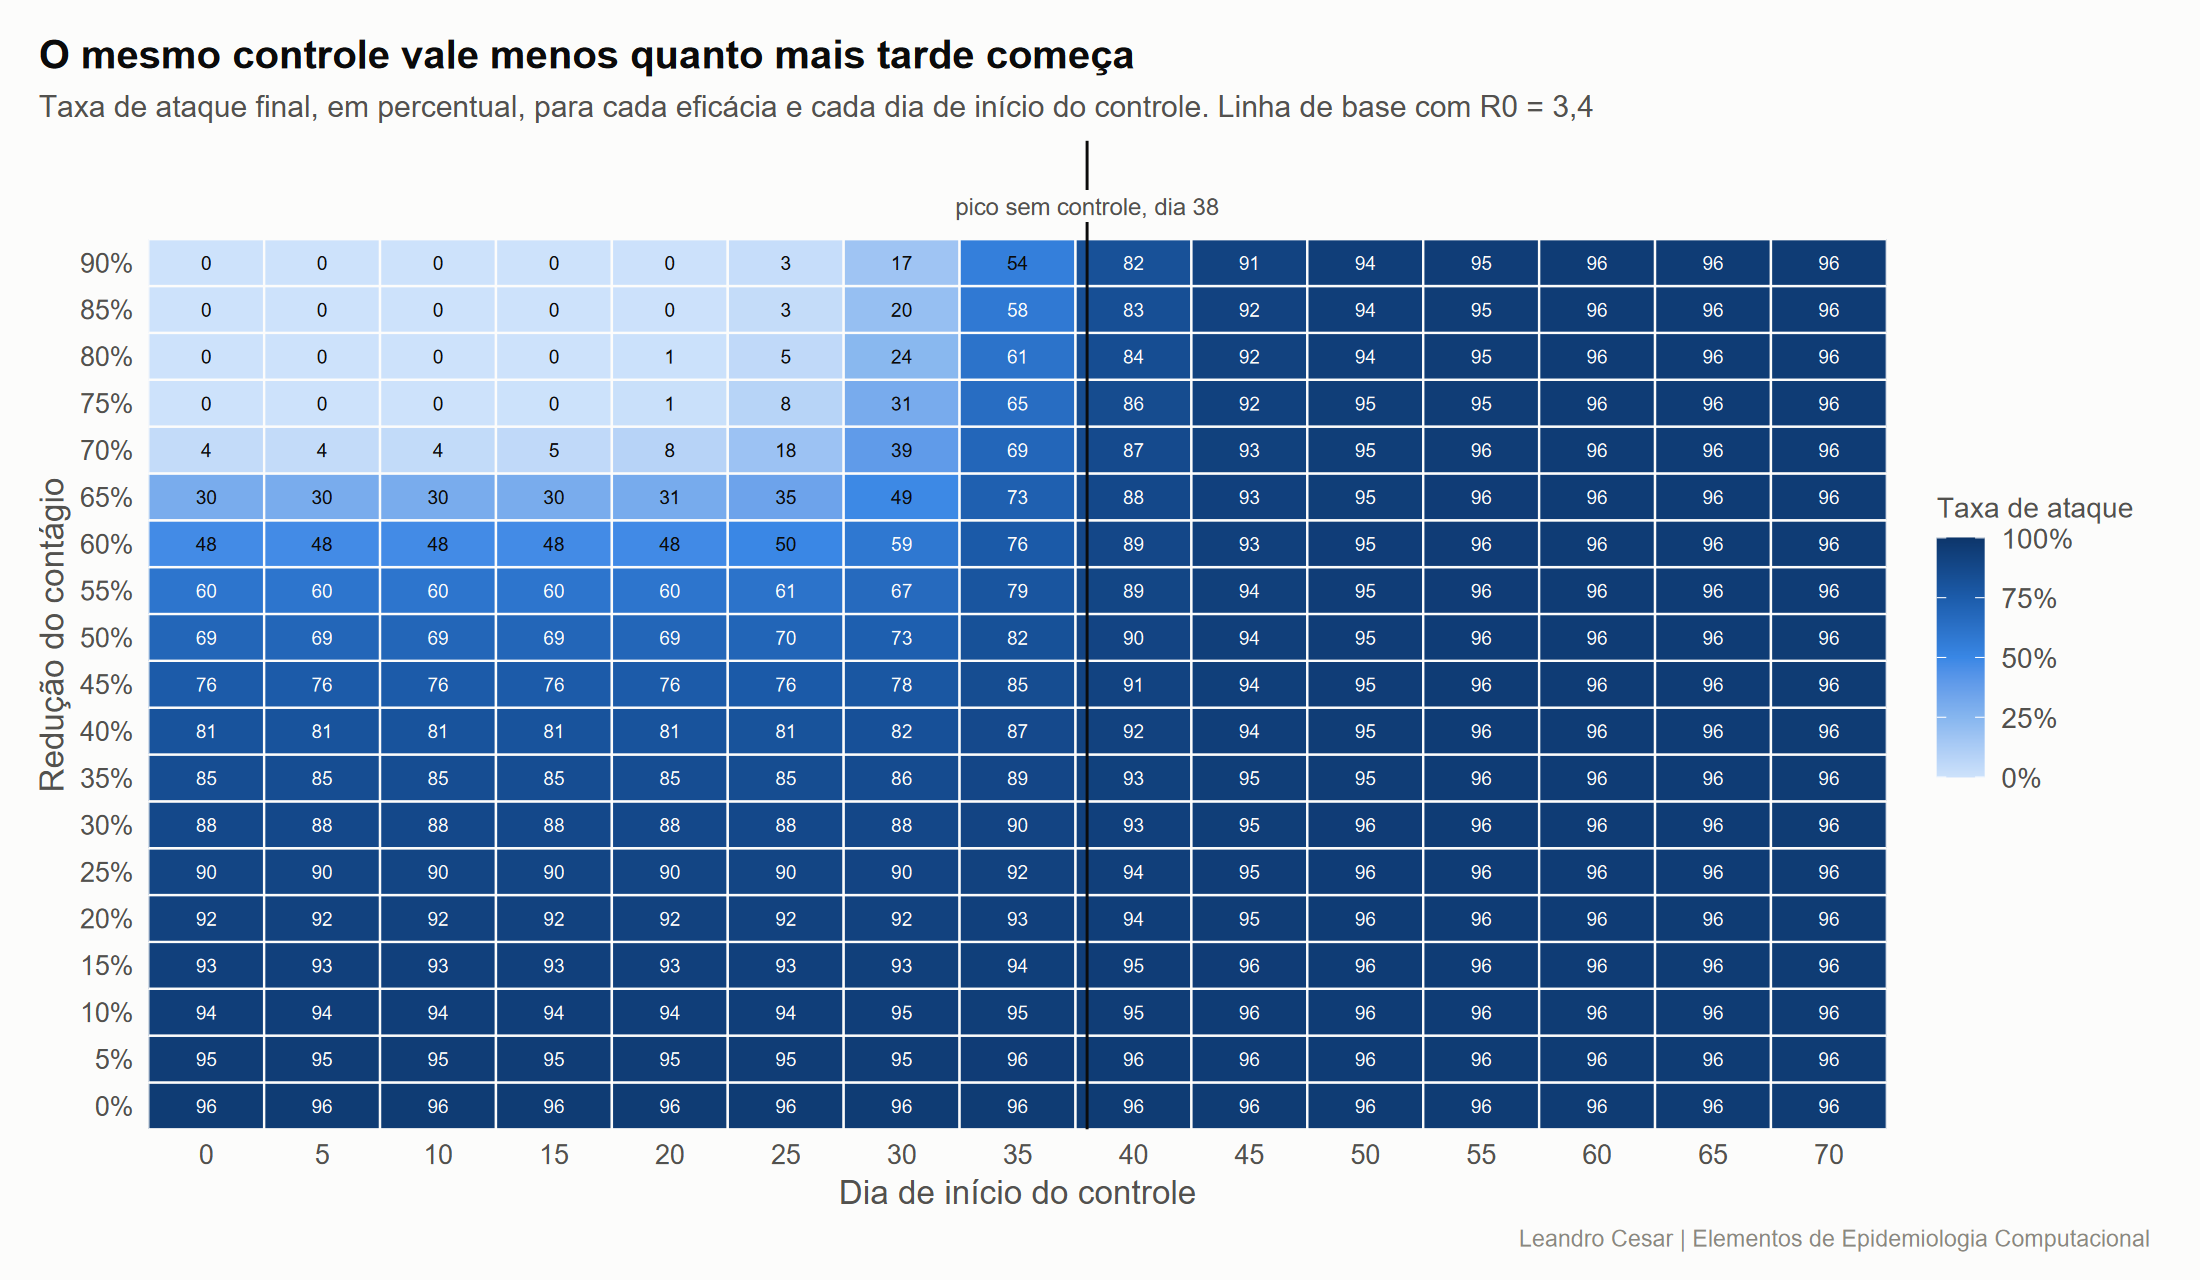
\includegraphics[width=0.95\textwidth]{fig10_controle_inicio.png}
\caption{Taxa de ataque final, em percentual, por eficácia e dia de início do controle no SIR.}
\label{fig:inicio}
\end{figure}

\paragraph{Reinfecção.} Para testar a hipótese de imunidade permanente, o SIR foi estendido com uma taxa de
perda de imunidade. Se a imunidade durasse em média 10 anos, uma segunda onda viria cerca de 6,7 anos
depois da primeira. Se durasse 2 anos, a doença ficaria endêmica, com cerca de 8.600 infectados a qualquer
momento. Nenhum dos dois quadros é necessário para explicar os dados do Recife, como mostra a discussão
abaixo, e a evidência imunológica sustenta a imunidade duradoura \cite{nitatpattana2014,
srikiatkhachorn2016, auerswald2018}.

\subsubsection{Os dados do Recife}

A Figura \ref{fig:dados} mostra a série de casos prováveis. A primeira onda começa em agosto de 2015 e tem
pico na semana de 14 de fevereiro de 2016, com 683 casos. A segunda, em 2021, chega a 1.319 casos na
semana de 30 de maio.

\begin{figure}[htbp]
\centering
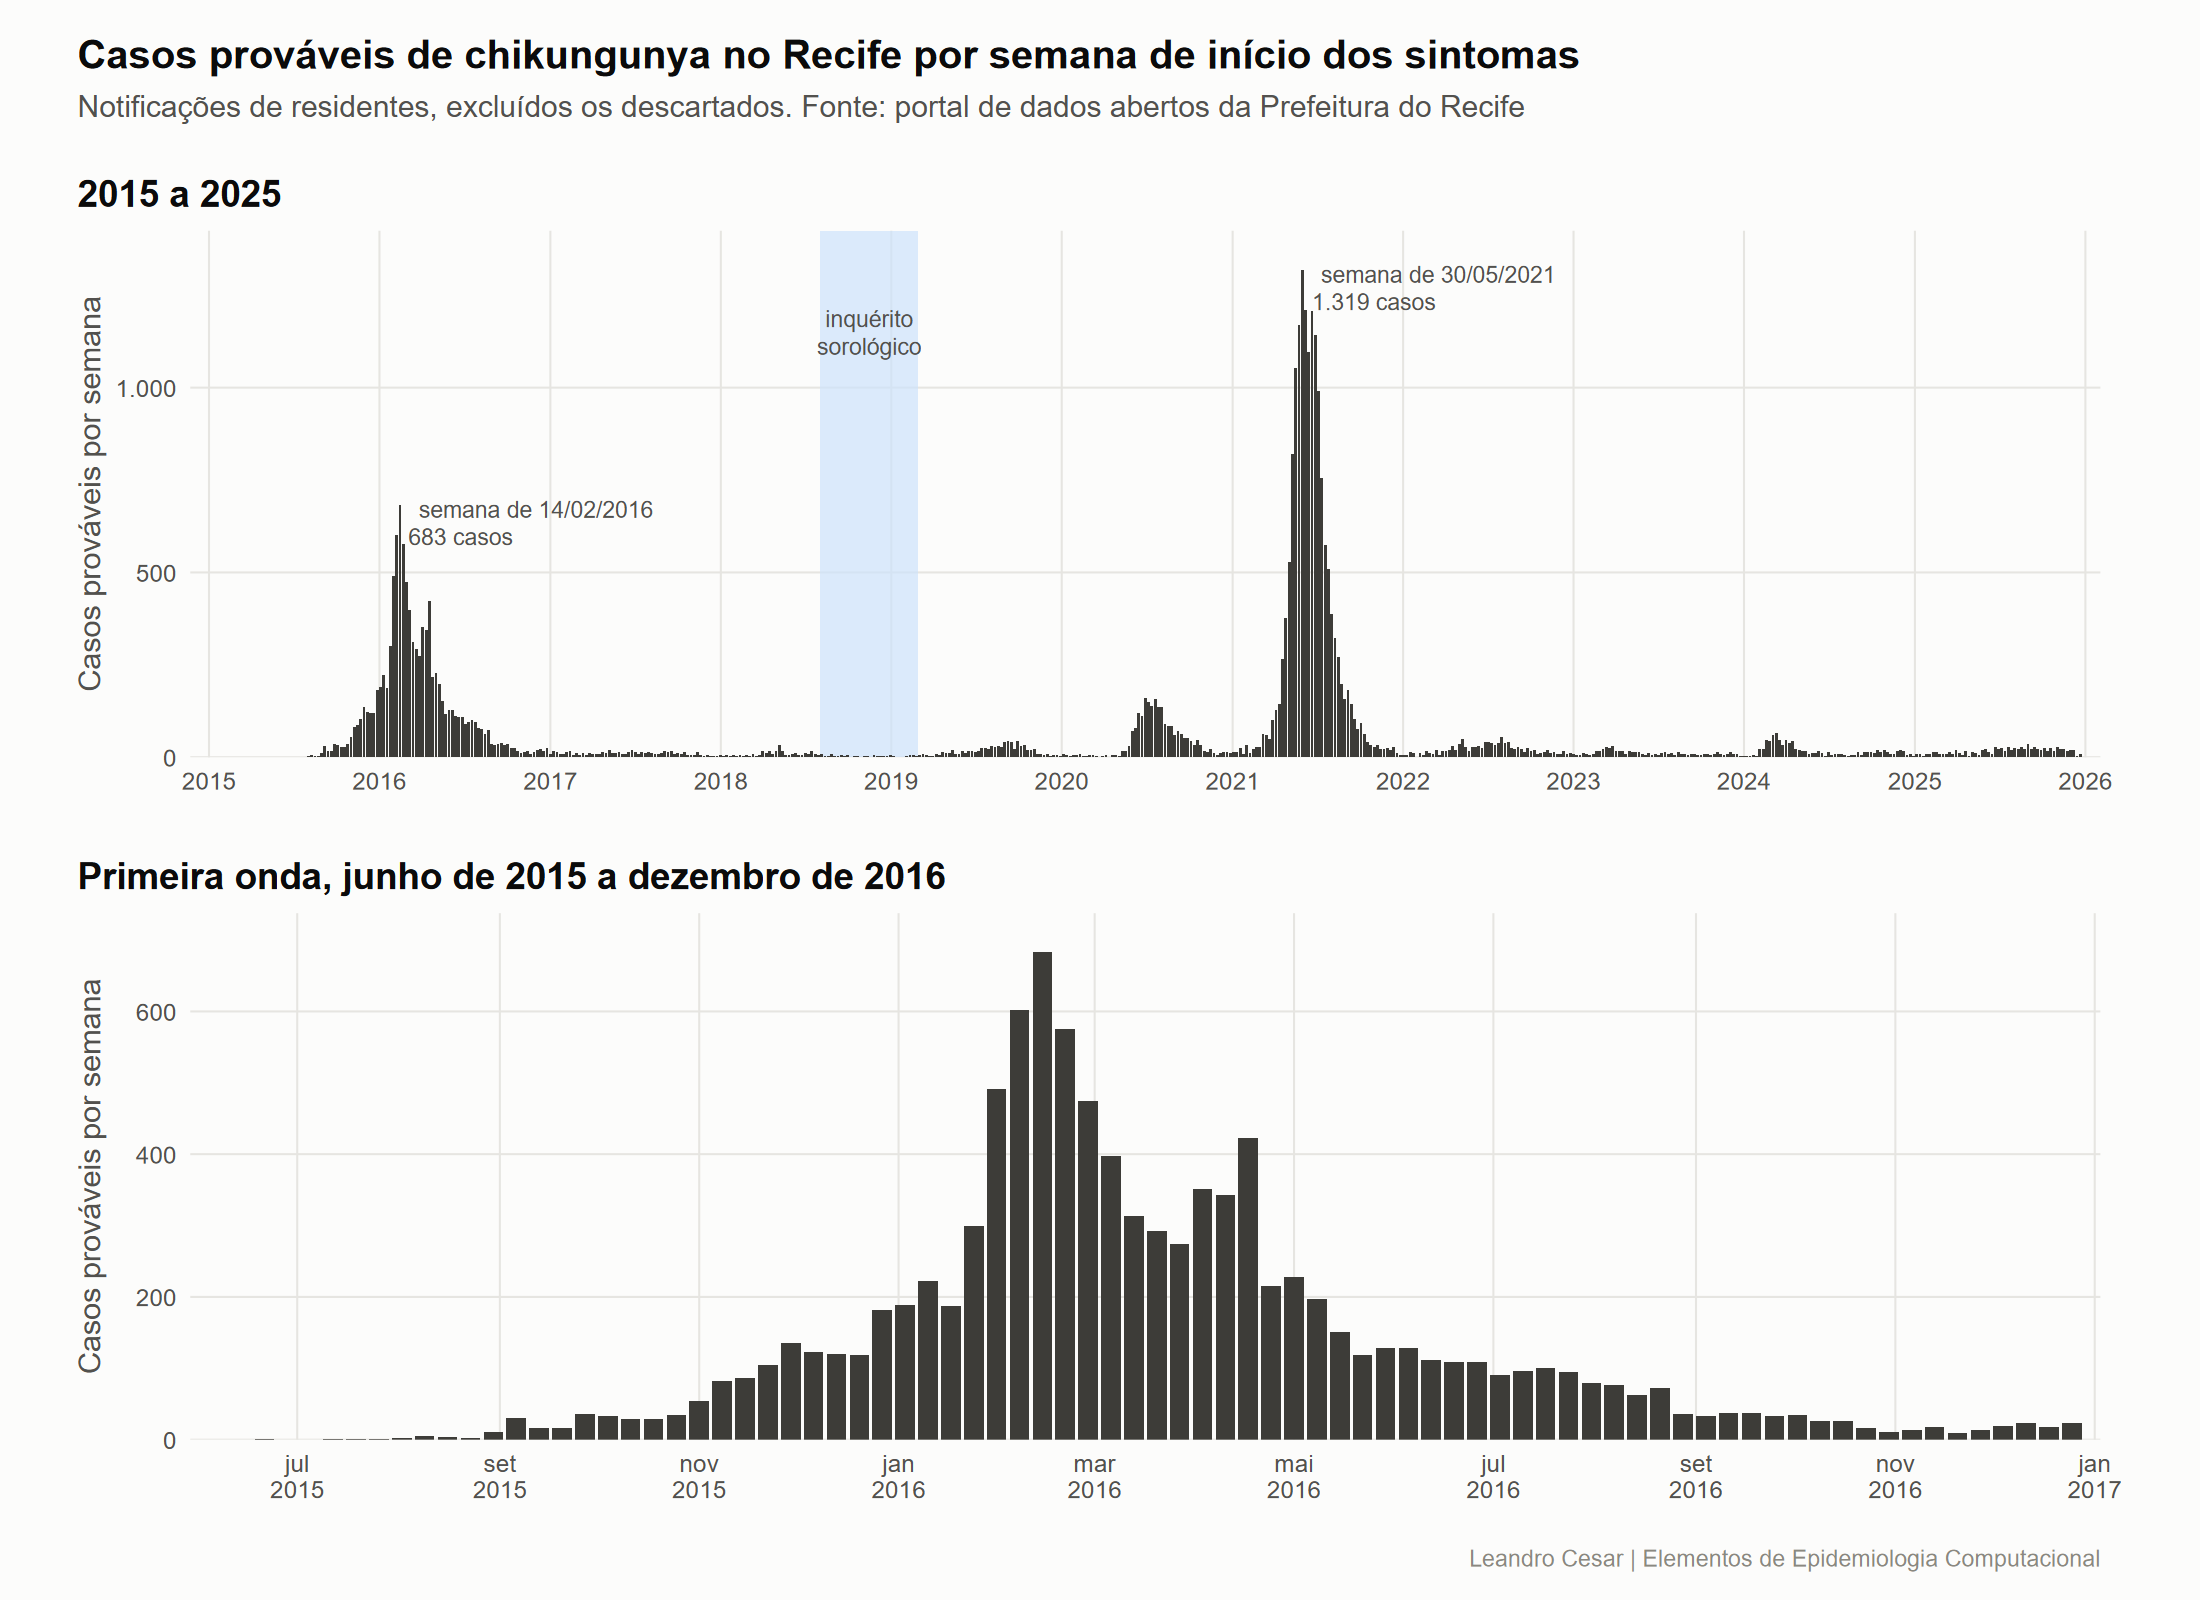
\includegraphics[width=\textwidth]{fig12_dados_recife.png}
\caption{Casos prováveis de chikungunya no Recife por semana de início dos sintomas.}
\label{fig:dados}
\end{figure}

Na fase de crescimento da primeira onda, de 30 de agosto de 2015 a 31 de janeiro de 2016, os casos
cresceram à taxa $r = 0{,}0208$ por dia (intervalo de confiança de 95\% de 0,0183 a 0,0232), dobrando a cada
33 dias (Figura \ref{fig:crescimento}). Cada modelo precisa de um número de reprodução diferente para
crescer nesse ritmo, porque cada um tem um intervalo de geração, o tempo entre uma infecção e a seguinte
na cadeia, diferente. No SIR, $r = \gamma(R_0 - 1)$ e portanto $R_0 = 1{,}12$. No SEIR-SEI, em que a geração
inclui a latência humana, a incubação no mosquito e a vida do mosquito, o valor exigido é $R_{hh} = 1{,}71$.
A Tabela \ref{tab:estimativas} reúne essas estimativas com a da literatura e a do inquérito.

\begin{figure}[htbp]
\centering
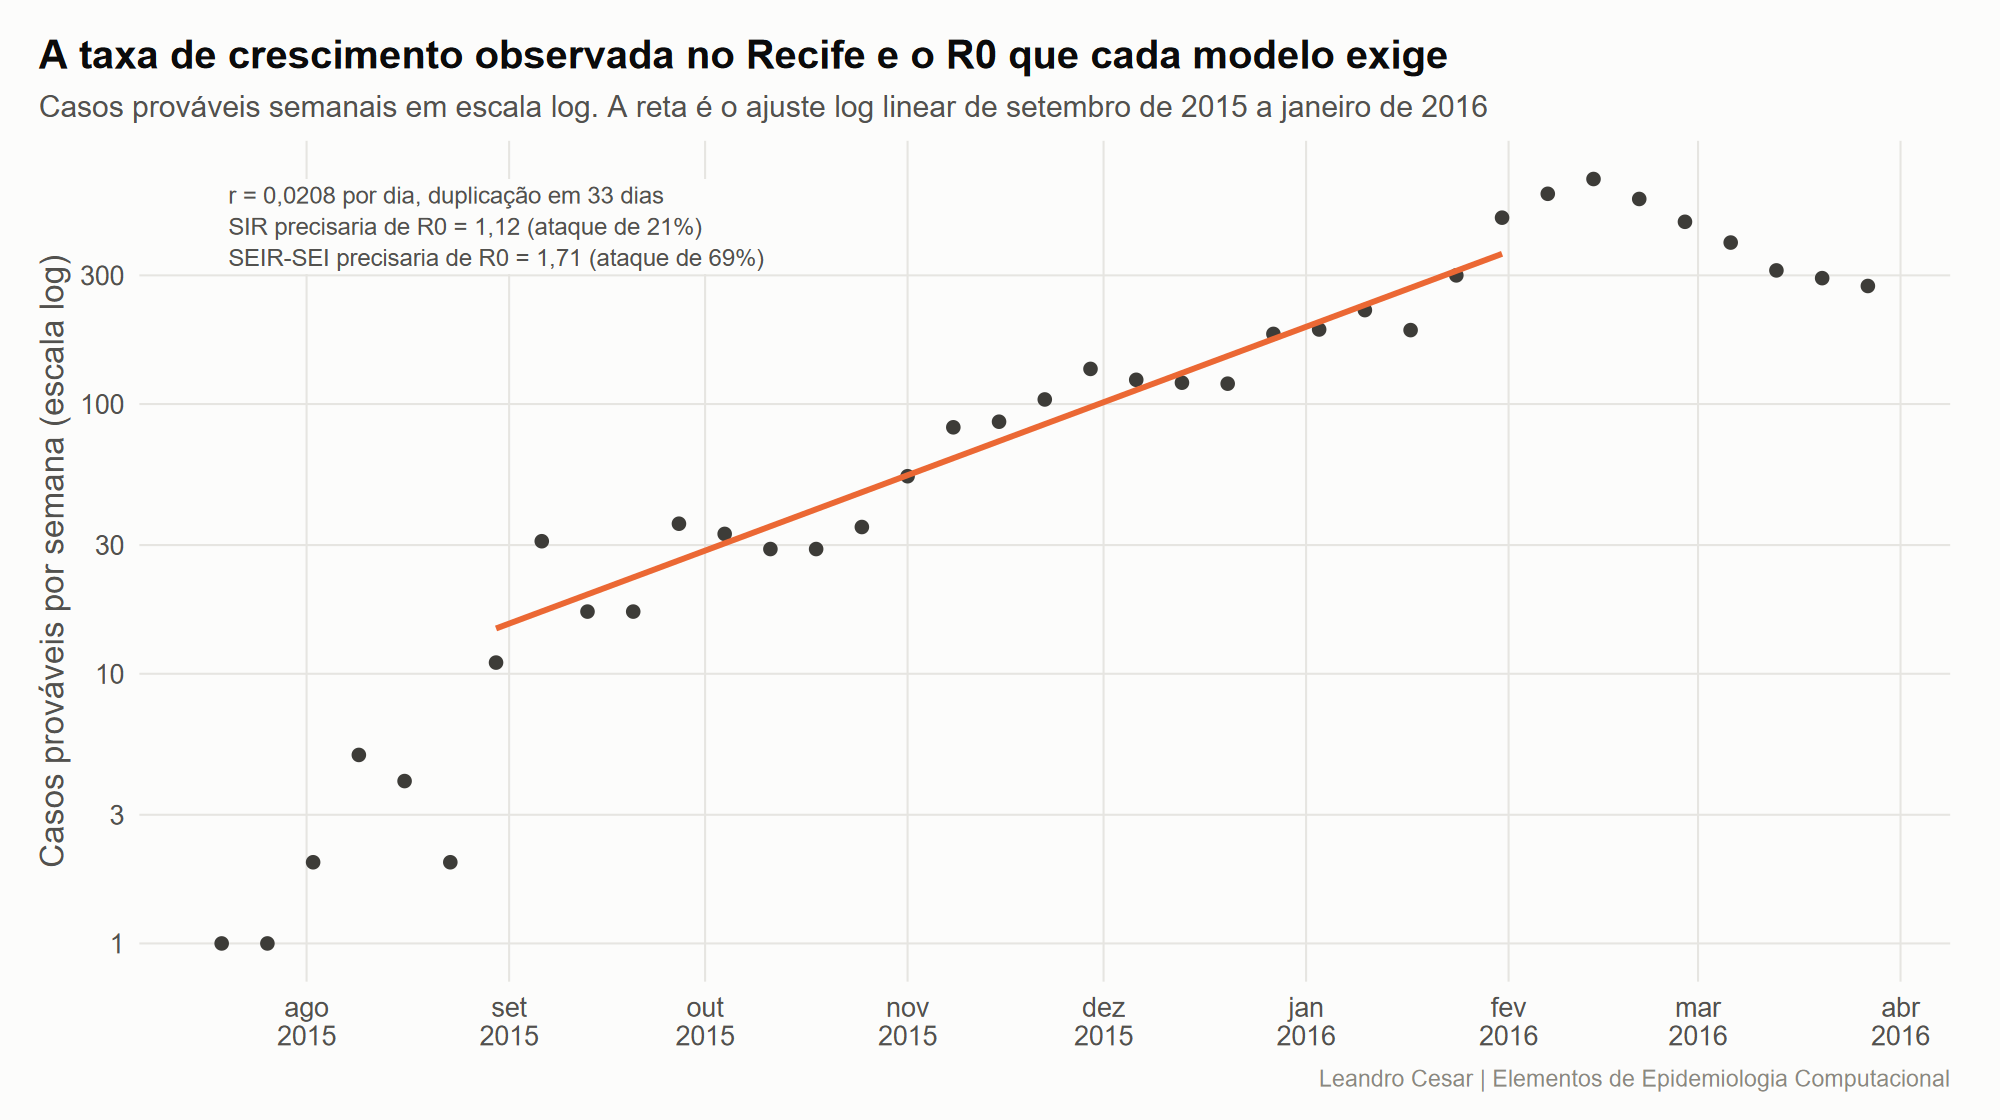
\includegraphics[width=0.92\textwidth]{fig13_crescimento_observado.png}
\caption{Taxa de crescimento da primeira onda, em escala logarítmica, e o $R_0$ que cada modelo exige.}
\label{fig:crescimento}
\end{figure}

\begin{table}[htbp]
\centering
\caption{Estimativas do número de reprodução de humano para humano e a taxa de ataque que cada uma implica
sob mistura homogênea.}
\label{tab:estimativas}
\small
\begin{tabular}{lcc}
\toprule
\textbf{Origem} & \textbf{$R_{hh}$} & \textbf{Taxa de ataque} \\
\midrule
Literatura \cite{haider2020} & 3,40 & 96\% \\
Crescimento observado, lido pelo SEIR-SEI & 1,71 & 69\% \\
Inquérito sorológico \cite{braga2023} & 1,24 & 36\% \\
Crescimento observado, lido pelo SIR & 1,12 & 21\% \\
\bottomrule
\end{tabular}
\end{table}

\subsubsection{O modelo SEIR-SEI}

Com o mesmo $R_{hh} = 3{,}4$, o SEIR-SEI cresce a 0,053 por dia, contra 0,40 do SIR, e o pico passa do dia 38
para o dia 271, com 115.189 infectados em vez de 515.090 (Figura \ref{fig:comparacao}). A taxa de ataque
quase não muda, 94,9\% contra 96,2\%, porque o tamanho final depende de $R_{hh}$. A ordem de grandeza do
tempo até o pico fica próxima da observada no Recife, cerca de seis meses, que o SIR erra por um fator de
cerca de cinco. A taxa de crescimento simulada, 0,0534 por dia, coincide com o autovalor do sistema
linearizado, 0,0533 por dia.

\begin{figure}[htbp]
\centering
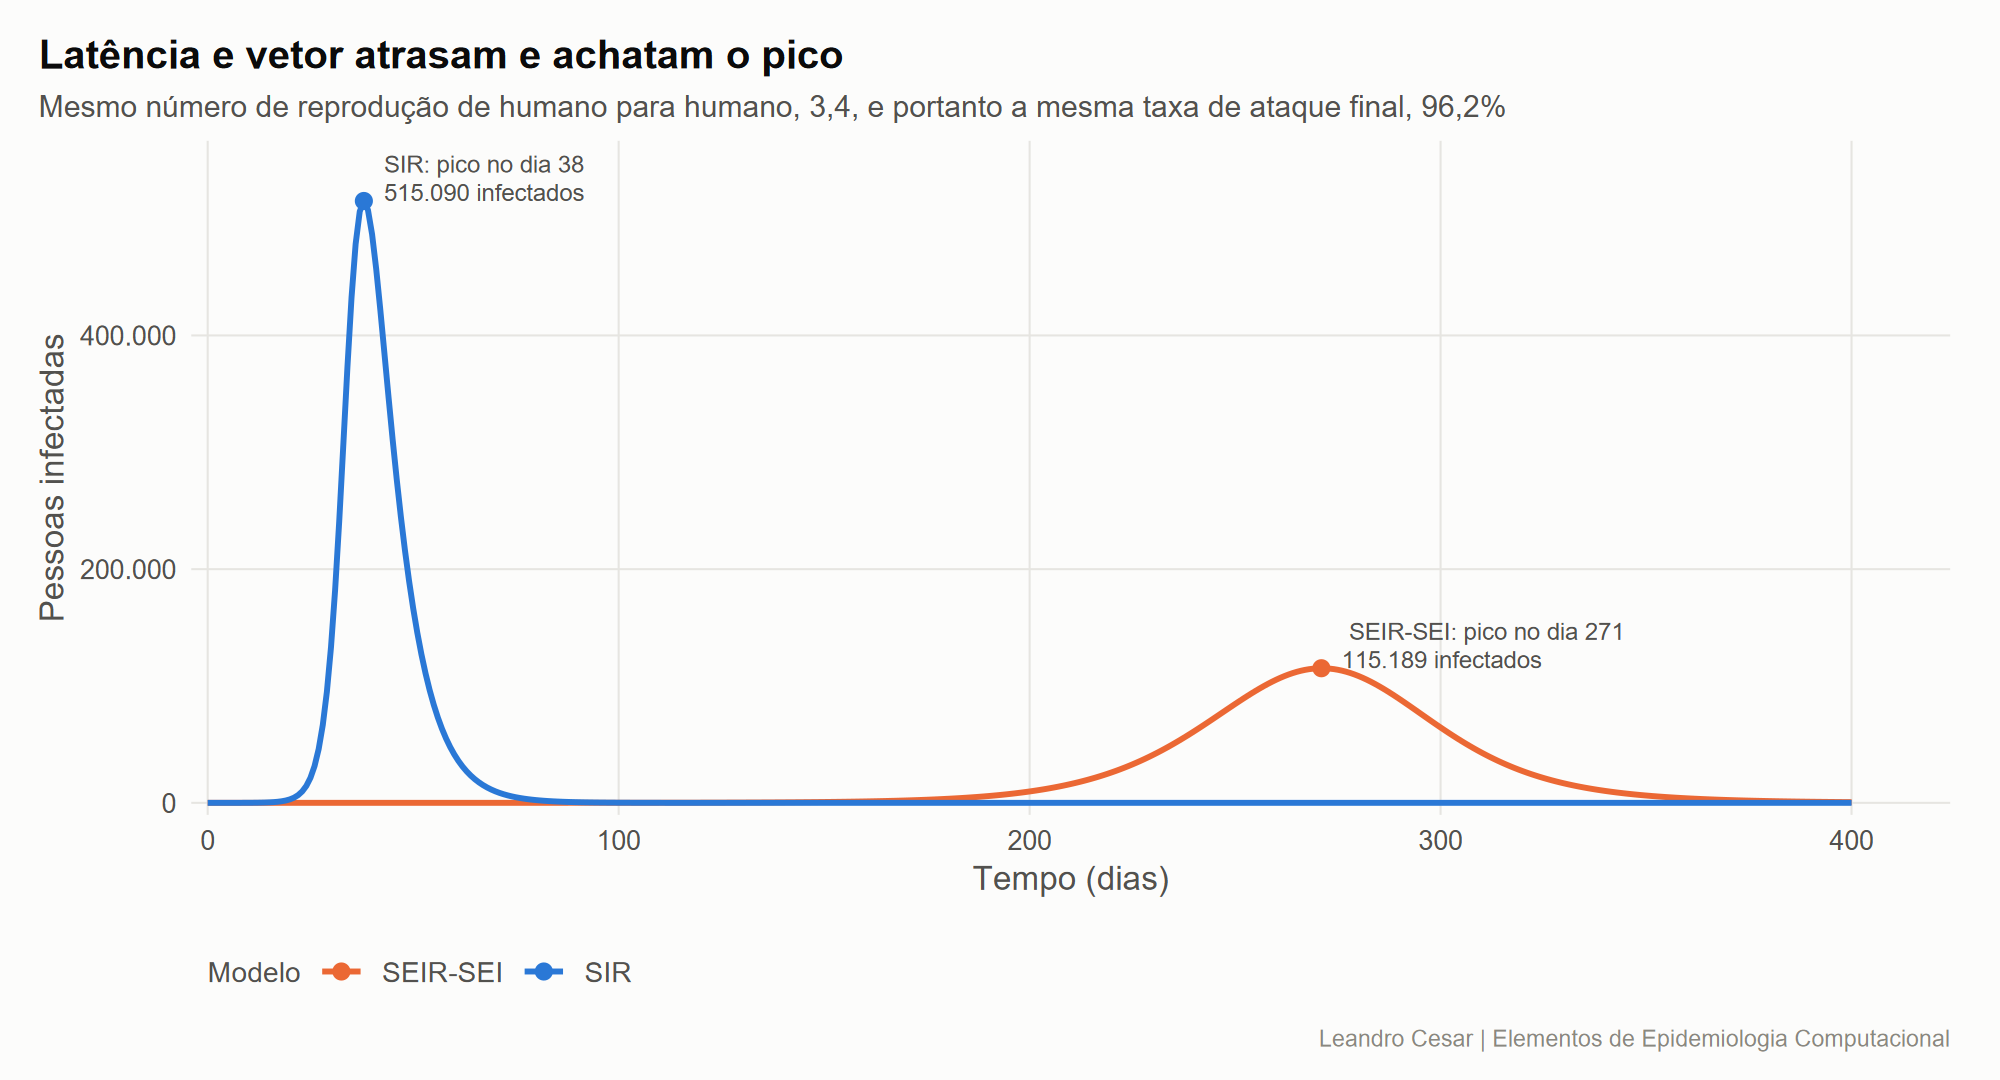
\includegraphics[width=0.92\textwidth]{fig16_sir_vs_seir_sei.png}
\caption{SIR e SEIR-SEI com o mesmo número de reprodução de humano para humano.}
\label{fig:comparacao}
\end{figure}

No SEIR-SEI, o controle de criadouros reduz o nascimento de mosquitos, e a população adulta só diminui à
medida que os mosquitos existentes morrem (Figura \ref{fig:controle}). Com redução de 80\%, os infectados
ainda crescem nas duas semanas seguintes ao início, e a taxa de ataque fica em 0,6\%, 25\% ou 76\% conforme
o controle comece no dia 120, 200 ou 250. A eficácia crítica é a mesma do SIR, $1 - 1/3{,}4 = 70{,}6\%$.
Quem usasse o $R_0$ de próxima geração, 1,84, calcularia $1 - 1/1{,}84 = 46\%$ e subestimaria o esforço
necessário, o que mostra por que a definição de $R_0$ precisa ser explícita.

\begin{figure}[htbp]
\centering
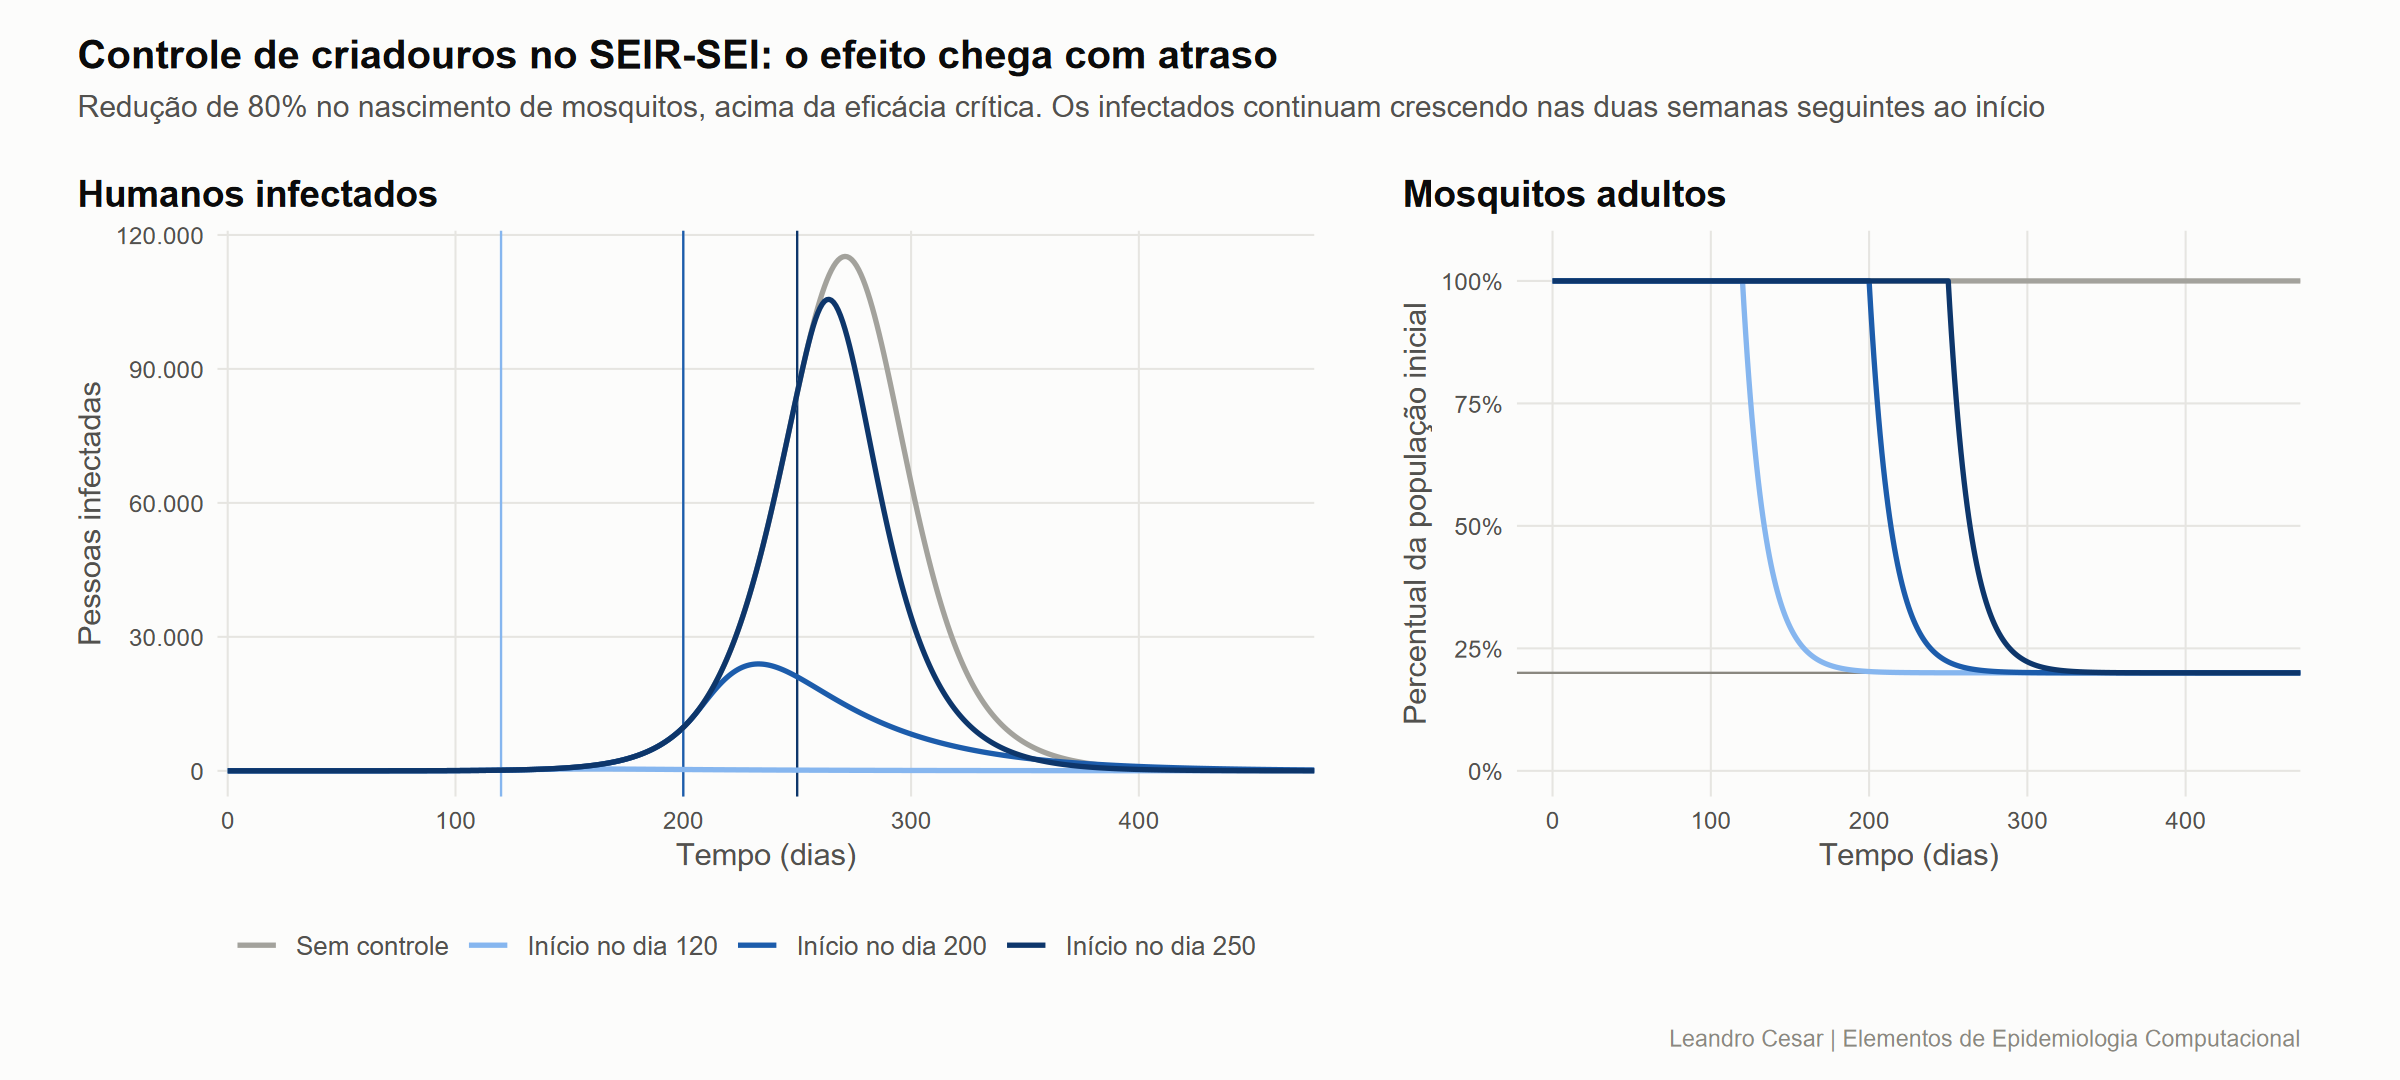
\includegraphics[width=\textwidth]{fig17_controle_vetorial.png}
\caption{Controle de criadouros no SEIR-SEI, iniciado em três momentos da fase de crescimento.}
\label{fig:controle}
\end{figure}

\subsubsection{Discussão dos resultados preliminares}

Os dados do Recife medem as distâncias entre os modelos homogêneos e a epidemia real em três frentes.

\textbf{Tamanho.} Com o $R_0$ da literatura, o SIR prevê que 96,2\% da população se infecte, e o inquérito
encontrou 35,7\% (Figura \ref{fig:sorologia}). Resolvendo a equação do tamanho final para $R_0$, os 35,7\%
correspondem a $R_0 = -\ln(1 - a)/a = 1{,}24$ sob mistura homogênea. A diferença entre o estrato alto,
22,3\%, e os demais, perto de 39\%, mostra que a cidade não se infectou por igual. Isso pesa contra a
mistura homogênea e é o que o OE4 vai testar.

\begin{figure}[htbp]
\centering
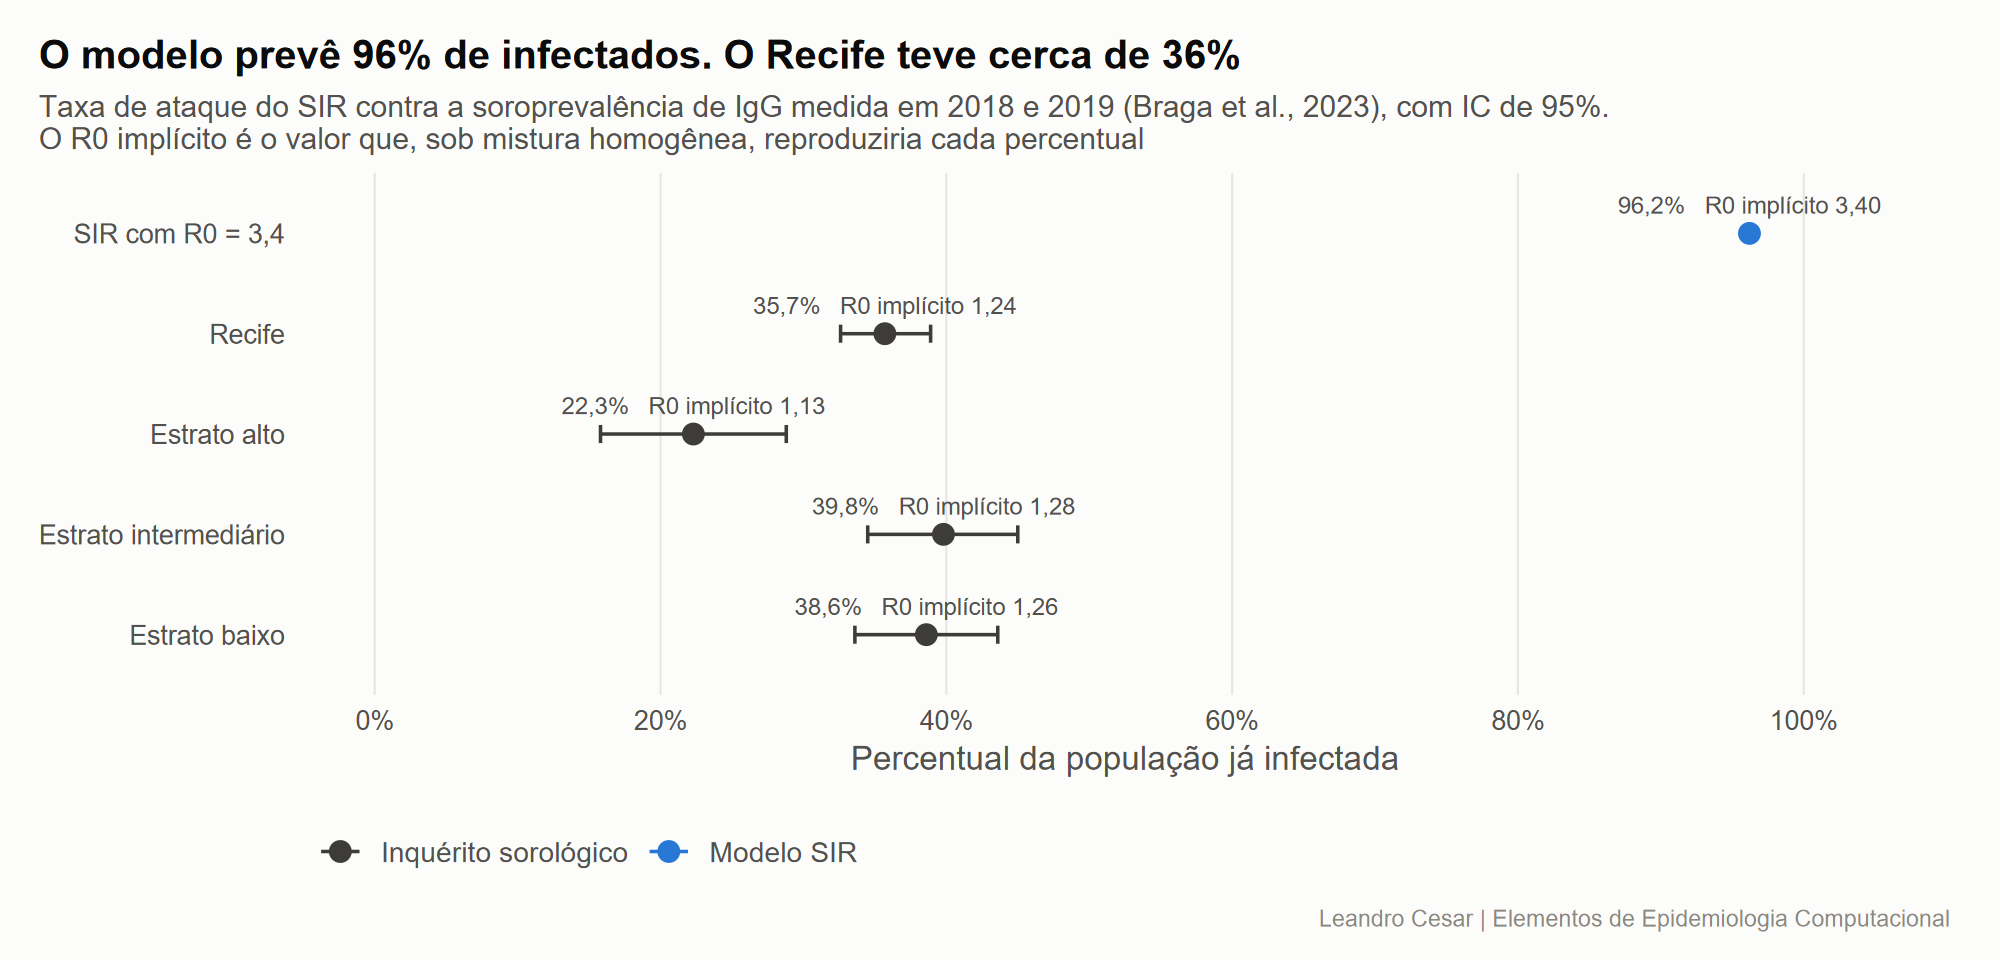
\includegraphics[width=0.92\textwidth]{fig14_sorologia.png}
\caption{Taxa de ataque do SIR contra a soroprevalência medida no Recife, com o $R_0$ implícito.}
\label{fig:sorologia}
\end{figure}

\textbf{Ritmo.} O SIR põe o pico 38 dias depois do primeiro caso, e a primeira onda levou cerca de seis
meses entre o início do crescimento e o pico. O SEIR-SEI corrige a ordem de grandeza, o que confirma a
sugestão de incluir o vetor e a latência. Como mostra a Tabela \ref{tab:estimativas}, a mesma série
observada implica números de reprodução diferentes em cada modelo: a estrutura do modelo não é um detalhe,
ela muda o que se conclui dos dados.

\textbf{Notificação.} Foram 9.989 casos prováveis em 2015 e 2016, 0,7\% da população. Se 35,7\% se
infectaram, foram cerca de 531 mil infecções, ou 53 para cada caso provável. \citeonline{braga2023} chegam a
uma razão parecida, de cerca de 45, com outra contagem de notificações. A fração de notificação, portanto,
precisa ser estimada junto com a transmissão, como prevê o OE3.

\textbf{Reinfecção ou heterogeneidade.} A onda de 2021 poderia sugerir perda de imunidade. Mas o inquérito,
feito antes dela, mostra que cerca de 64\% da população nunca tinha sido infectada, o que basta para uma nova
onda sem reinfecção. A hipótese mais simples é que a primeira onda parou antes de atingir toda a cidade,
por causa da estação e da distribuição desigual da transmissão entre os grupos.

Nenhum modelo homogêneo reproduz ao mesmo tempo a velocidade e o tamanho da primeira onda: o SEIR-SEI,
ajustado pelo crescimento, ainda prevê 69\% de infectados. A diferença que sobra é o objeto da proposta. Há
também limitações nos dados que o projeto precisa enfrentar: o significado dos códigos antigos de
classificação, e o fato de que parte do crescimento inicial das notificações pode refletir a atenção
crescente dos serviços a uma doença nova, e não só a transmissão.

\subsection{Aspectos éticos}

A pesquisa é computacional e usa apenas dados secundários: as notificações publicadas no portal de dados
abertos da Prefeitura do Recife \cite{recife2026}, a população do Censo 2022 e os resultados agregados
publicados do inquérito sorológico. Não há contato com participantes. Os arquivos do portal são públicos,
mas trazem campos que permitem identificar pessoas, como endereço e data de nascimento. Por isso esses
arquivos são guardados apenas localmente, fora do repositório, e o projeto usa e publica somente contagens
agregadas por semana e por distrito, sem possibilidade de identificação individual. A Resolução CNS
510/2016 dispensa de registro no sistema CEP/CONEP a pesquisa com informações de acesso público e a
pesquisa com bancos de dados de informações agregadas \cite{cns510}. Como o tratamento parte de registros
individuais, antes da execução a dispensa será confirmada com o Comitê de Ética em Pesquisa da UFRPE,
considerando também a Resolução CNS 738/2024, que trata do uso de bancos de dados em pesquisa
\cite{cns738}.
